\section*{Albert Einstein\protect\footnote{\url{https://en.wikipedia.org/wiki/Albert_Einstein}}}

\begin{figure}[ht]
  \centering
  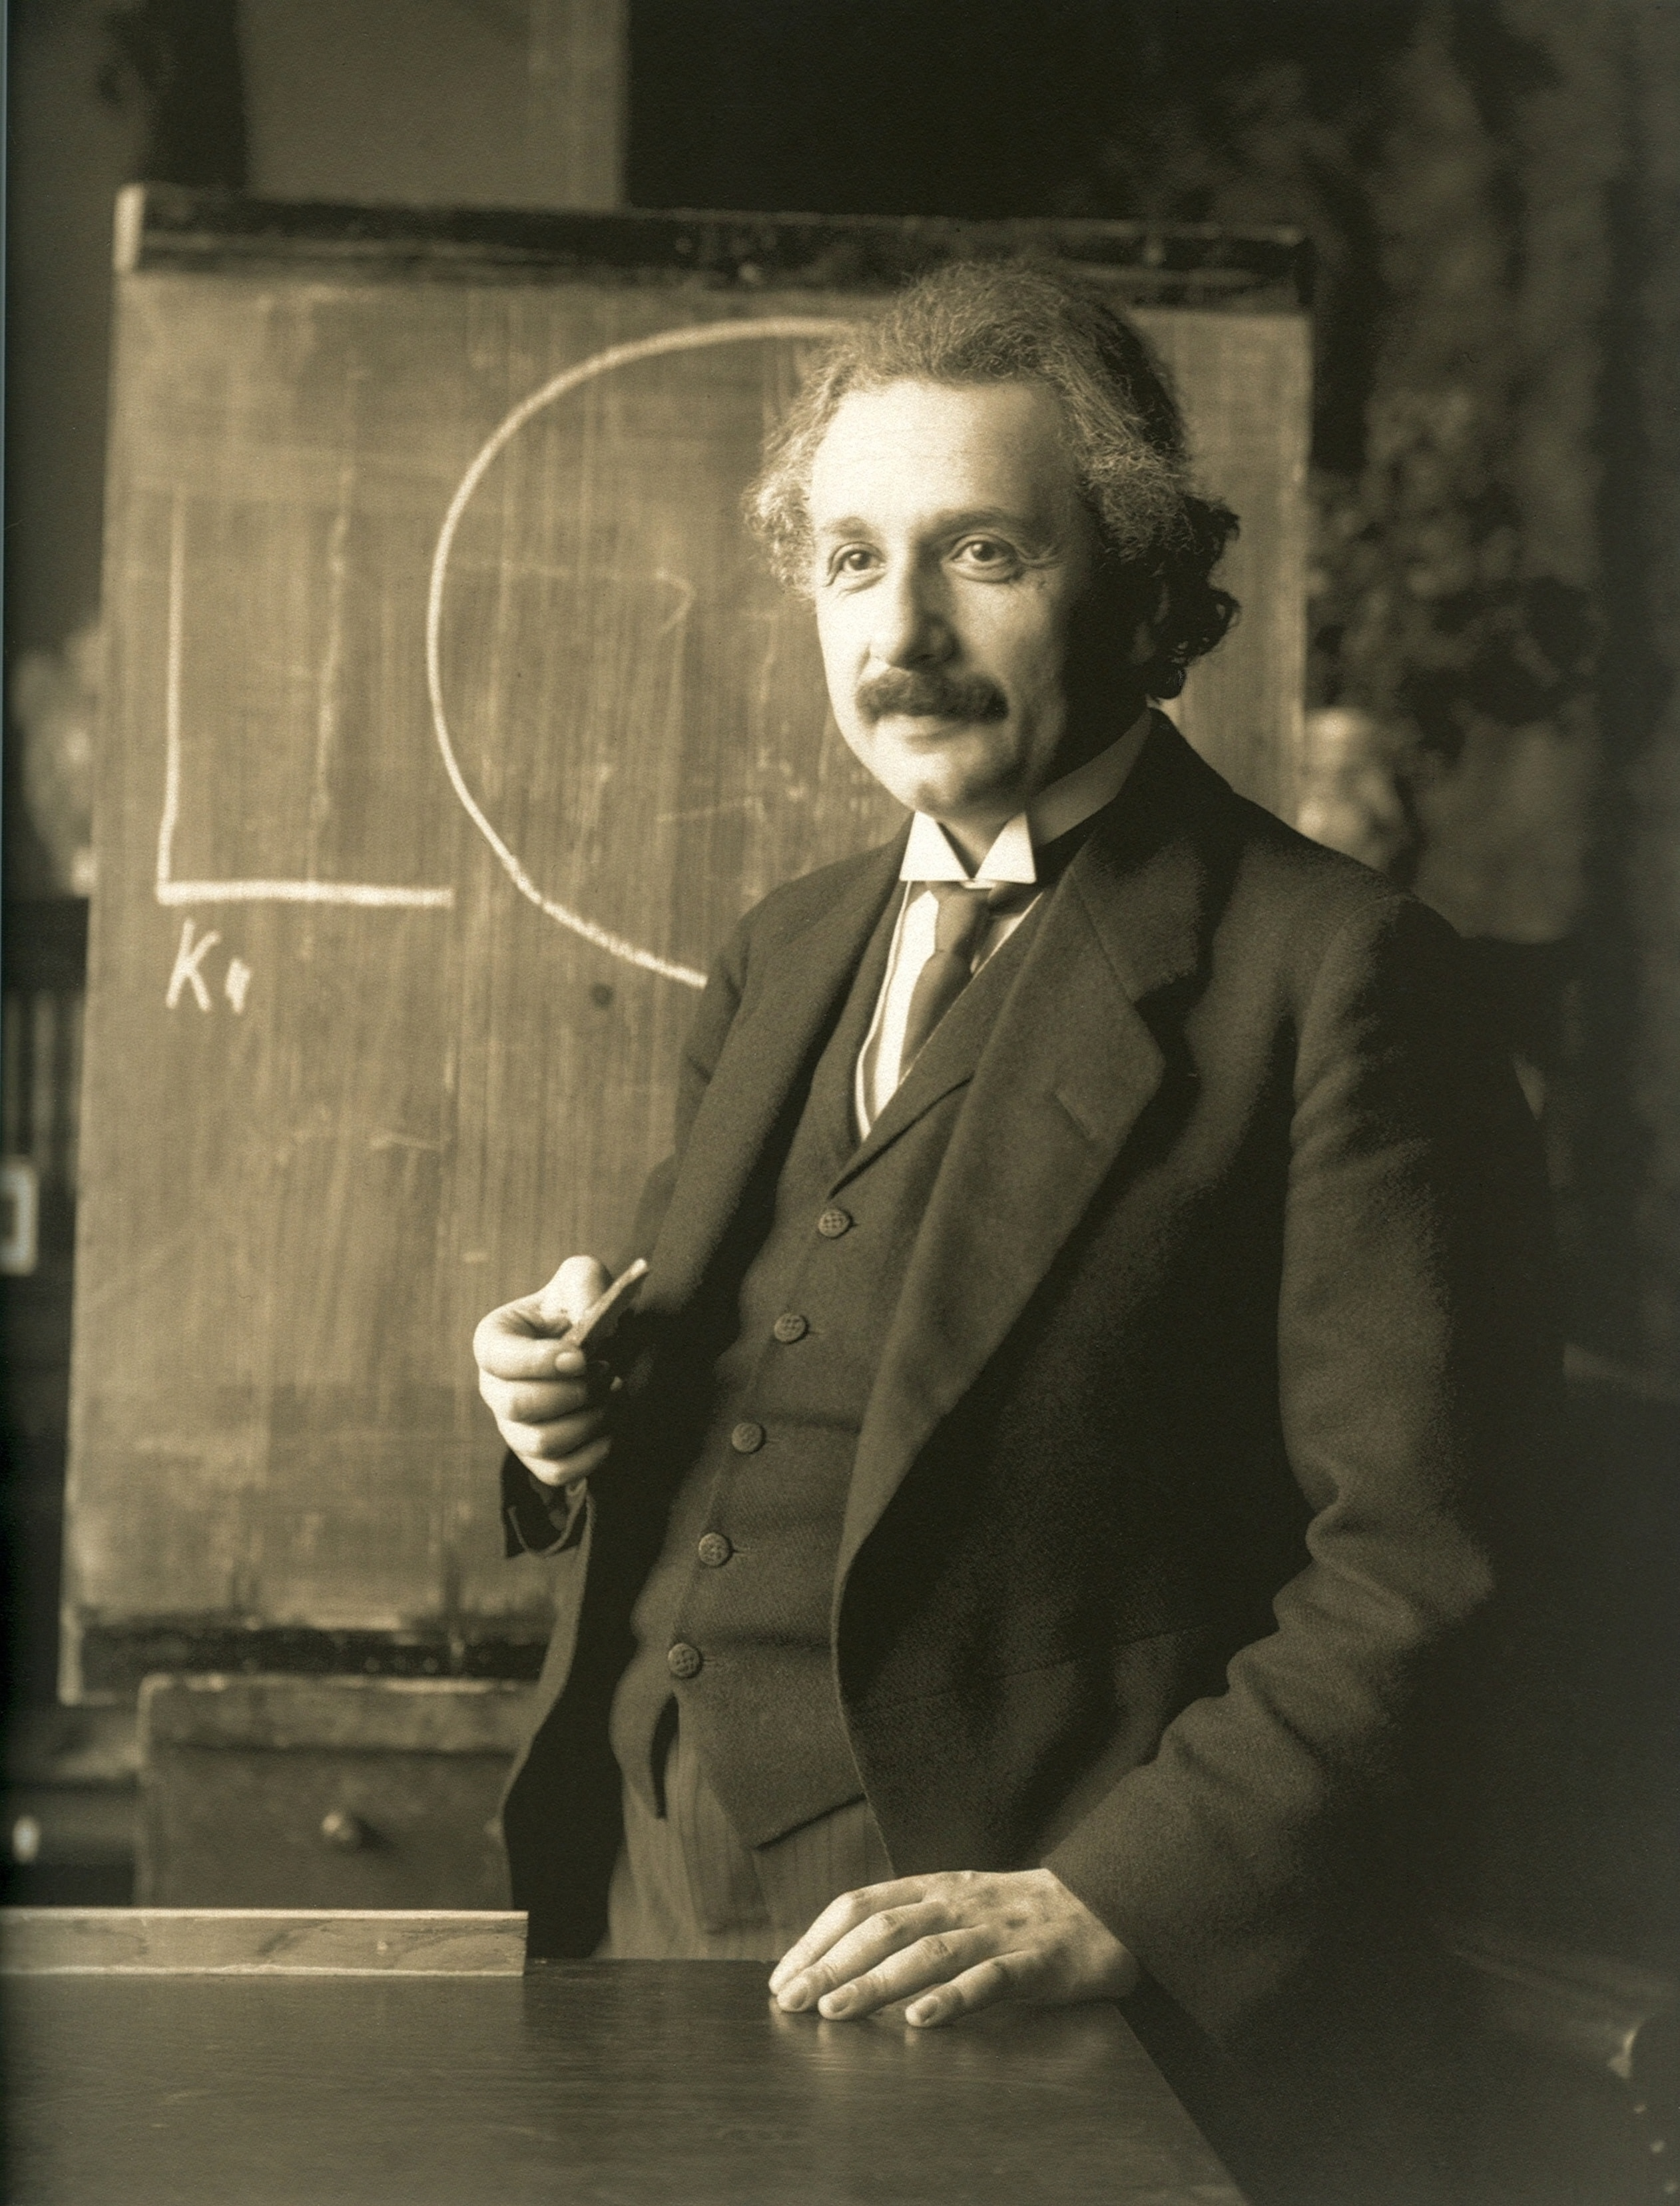
\includegraphics[width=0.8\linewidth]{content/figures/albert_einstein_picuture.jpg}
  \caption{Albert Einstein in 1921\protect\footnotemark}
\end{figure}
\footnotetext{\url{https://commons.wikimedia.org/wiki/File:Einstein_1921_by_F_Schmutzer_-_restoration.jpg}}

Albert Einstein (14 March 1879 – 18 April 1955) was a German-born theoretical physicist. He developed the theory of relativity, one of the two pillars of modern physics (alongside quantum mechanics). Einstein's work is also known for its influence on the philosophy of science. Einstein is best known in popular culture for his mass–energy equivalence formula $E = mc^2$ (which has been dubbed ``the world's most famous equation''). He received the 1921 Nobel Prize in Physics ``for his services to theoretical physics, and especially for his discovery of the law of the photoelectric effect'', a pivotal step in the evolution of quantum theory.

Near the beginning of his career, Einstein thought that Newtonian mechanics was no longer enough to reconcile the laws of classical mechanics with the laws of the electromagnetic field. This led him to develop his special theory of relativity during his time at the Swiss Patent Office in Bern (1902–1909), Switzerland. He realized, however, that the principle of relativity could also be extended to gravitational fields, and with his subsequent theory of gravitation in 1916, he published a paper on general relativity. He continued to deal with problems of statistical mechanics and quantum theory, which led to his explanations of particle theory and the motion of molecules. He also investigated the thermal properties of light which laid the foundation of the photon theory of light. In 1917, Einstein applied the general theory of relativity to model the large-scale structure of the universe.

Between 1895 and 1914 he lived in Switzerland (except for one year in Prague, 1911–12), where he received his academic diploma from the Swiss Federal Polytechnic in Zürich (later the Eidgenössische Technische Hochschule, ETH) in 1900. He later taught there at the same institute as a professor of theoretical physics between 1912 and 1914 before he left for Berlin. In 1901, after being stateless for more than five years, Einstein acquired Swiss citizenship, which he kept for the rest of his life. In 1905, Einstein was awarded a PhD by the University of Zürich. The same year, his annus mirabilis (miracle year), he published four groundbreaking papers, which were to bring him to the notice of the academic world, at the age of 26.

He was visiting the United States when Adolf Hitler came to power in 1933 and, being Jewish, did not go back to Germany, where he had been a professor at the Berlin Academy of Sciences. He settled in the United States, becoming an American citizen in 1940. On the eve of World War II, he endorsed a letter to President Franklin D. Roosevelt alerting him to the potential development of ``extremely powerful bombs of a new type'' and recommending that the U.S. begin similar research. This eventually led to what would become the Manhattan Project. Einstein supported defending the Allied forces, but generally denounced the idea of using the newly discovered nuclear fission as a weapon. Later, with the British philosopher Bertrand Russell, Einstein signed the Russell–Einstein Manifesto, which highlighted the danger of nuclear weapons. Einstein was affiliated with the Institute for Advanced Study in Princeton, New Jersey, until his death in 1955.

Einstein published more than 300 scientific papers along with over 150 non-scientific works. On 5 December 2014, universities and archives announced the release of Einstein's papers, comprising more than 30,000 unique documents. Einstein's intellectual achievements and originality have made the word ``Einstein'' synonymous with ``genius''.
